\section{Implementation}

\subsection{Implementation Details}

Figures \ref{fig:Detectionofdesignantipatterns}, \ref{fig:Detectionoflinguisticquality}, \ref{fig:Puttingtogetherthefindings}, \ref{fig:Rchisquarecalculation}, and \ref{fig:Calculationofphicoefficients} illustrates programs created and used for our research.

\begin{figure}[h!]
 \centering
 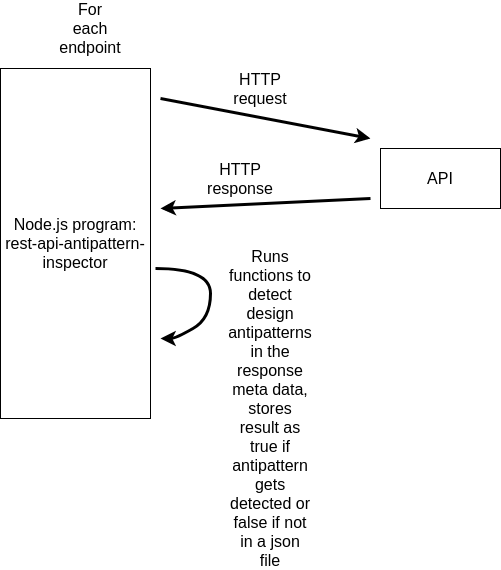
\includegraphics[scale=0.5]{img/method_figures/rest-api-antipattern-inspector.png}
 \caption{Detection of design antipatterns.}
 \label{fig:Detectionofdesignantipatterns}
\end{figure}

\begin{figure}[h!]
 \centering
 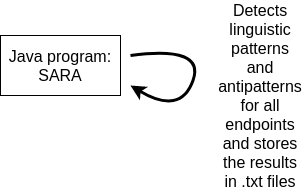
\includegraphics[scale=0.55]{img/method_figures/JAVA_SARA.png}
 \caption{Detection of linguistic quality.}
 \label{fig:Detectionoflinguisticquality}
\end{figure}

\begin{figure}[h!]
 \centering
 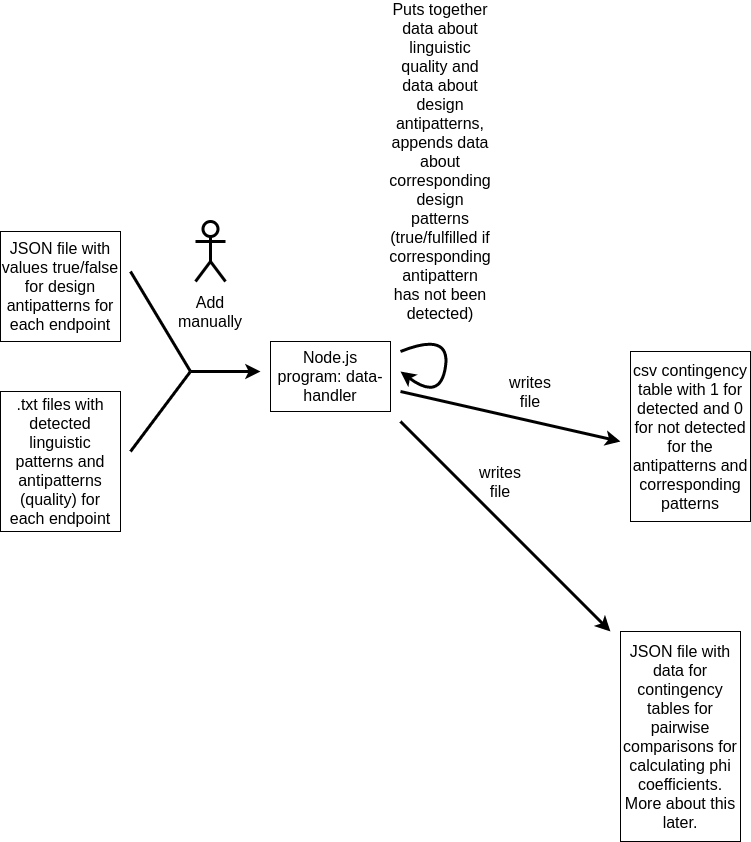
\includegraphics[scale=0.45]{img/method_figures/data_handler.png}
 \caption{Putting together the findings.}
 \label{fig:Puttingtogetherthefindings}
\end{figure}

\begin{figure}[h!]
 \centering
 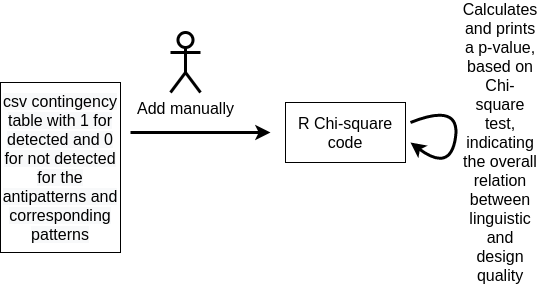
\includegraphics[scale=0.5]{img/method_figures/R_Chi_square.png}
 \caption{Chi square calculation.}
 \label{fig:Rchisquarecalculation}
\end{figure}

\begin{figure}[h!]
 \centering
 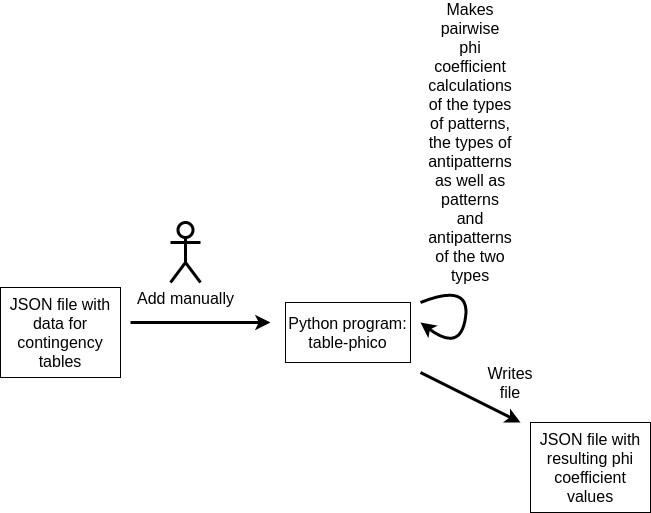
\includegraphics[scale=0.5]{img/method_figures/table_phico.png}
 \caption{Calculation of Phi coefficients.}
 \label{fig:Calculationofphicoefficients}
\end{figure}

\clearpage

\subsection{Detection of Linguistic Antipatterns}

SARA (Semantic Analysis of RESTful APIs) is a Java program used for the detection of Linguistic Quality in URIs of REST APIs introduced by Palma et al. \cite{linguistic}. 

Our research will use SARA \cite{linguistic} for detecting the following linguistic antipatterns:
\begin{itemize}
\item Amorphous URIs
\item CRUDY URIs
\item Non-hierarchical Nodes
\item Inconsistent use of Singularised/Pluralised Nodes
\item Contextless Resource Names
\end{itemize}

%The following antipatterns can be detected with SARA but will be excluded from our research.
%\begin{itemize}
%\item Unversioned URIs - If an API in is not versioning their URIs there will be an effect on all the endpoints in that API. We think it is to difficult to draw a conclusion that there could be a relation with design quality.
%\item Inconsistent documentation - we want to focus on the structure of the URIs in question and not the documentation written about them.
%\item Less cohesive documentation -  see %above.
%\end{itemize}

SARA is built on JAVA and runs in the console. Each API is run separately and the result is stored in text files. Each text file consists of a list with URIs that are antipatterns and URI that passed the test.
The linguistic program has been further developed to get a more accurate result from finding context-less resources/URIs. Previously there was a limitation where nodes in a URI had words written together like `districtheat' where the following URI would become an antipattern: 

\vspace{2mm}
\texttt{/v3/{agreementId}/consumption/districtheat/data}

\vspace{2mm}
With our improvement, the program can detect words written together and treat them as separate nodes. If a word is not found in the dictionary then this code block is executed to check if the word might consist of more than one word. The two new words must make use of all the characters of the old word.

\subsection{Detection of REST Design Antipatterns}

To be able to detect REST design antipatterns in APIs, we have developed a program for automatically making API calls, analyzing the metadata and storing the results. 
The program for detecting REST design antipatterns is written in TypeScript using the Node.js platform. These techniques were chosen partly because JavaScript is the most used language on GitHub \cite{octogithub} and because TypeScript, which extends JavaScript \cite{typescript}, is among the fastest growing languages on GitHub \cite{octogithub}. The aim is that this choice of techniques will help make our source code understandable for a wide audience. It is desirable for the sake of increased reliability for other developers and researchers to be able to understand our source code and thereby be able to validate it. Working with techniques that are currently commonly used will also result in access to many modern third party software libraries which will simplify and speed up the development process as well as reduce the risk of flaws since software libraries that are commonly used, have been battle-tested and have gotten good reviews can be selected. In addition, Node.js was selected for its suitability for handling HTTP calls \cite{nodejs} and TypeScript was selected to help with the detection of flaws \cite{typescript} in the development of the source code. 
The program has a Command Line Interface (CLI), the user selects which APIs to run detection for and the results with meta data gets stored in a JSON file \footnote{\url{https://github.com/rest-api-antipattern-inspector/rest-api-antipattern-inspector}}. 

\subsection{Design Antipattern Detection Functions}

Figures \ref{fig:BreakingSelf-descriptiveness}, \ref{fig:ForgettingHypermedia}, \ref{fig:IgnoringCaching}, \ref{fig:IgnoringMIMETypes}, \ref{fig:IgnoringStatusCode}, and \ref{fig:MisusingCookies} show the source code for functions we have created to detect REST design antipatterns. Many of these functions use helper functions we have created in other parts of the source code, it returns the boolean value true if the antipattern is detected and false otherwise.

As shown in Figure \ref{fig:BreakingSelf-descriptiveness}, the Breaking Self-descriptiveness antipattern gets detected if there are any non-standard headers in the request or response headers after an API call.

\begin{figure}[h!]
 \centering
 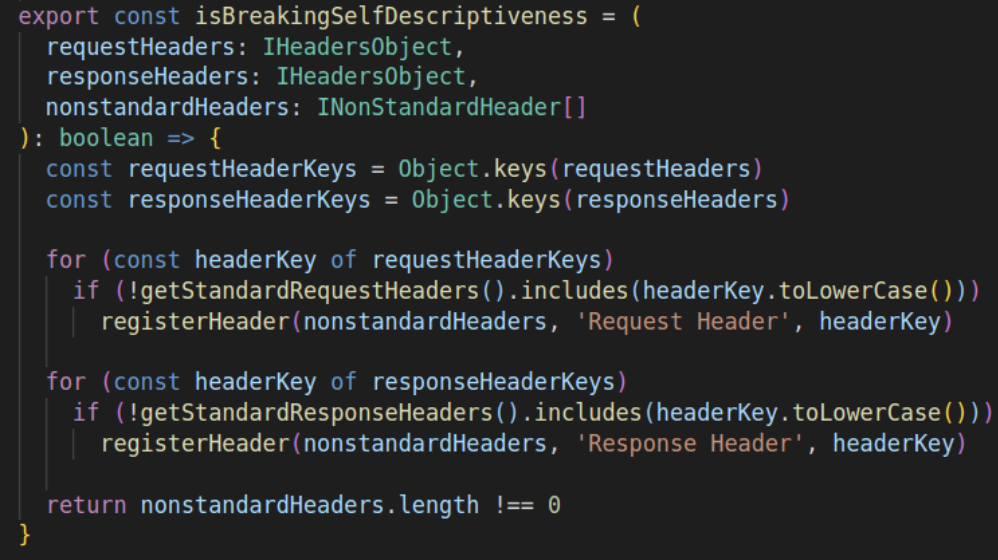
\includegraphics[width=0.8\textwidth]{img/breakingSelfDescriptiveness.png}
 \caption{The detection of Breaking Self-descriptiveness.}
 \label{fig:BreakingSelf-descriptiveness}
\end{figure}

As shown in Figure \ref{fig:ForgettingHypermedia}, the Forgetting Hypermedia antipattern gets detected if the response body to a GET request does not contain any link keys (link/links/href) or if a POST request does not contain that or a Location header.

\begin{figure}[h!]
 \centering
 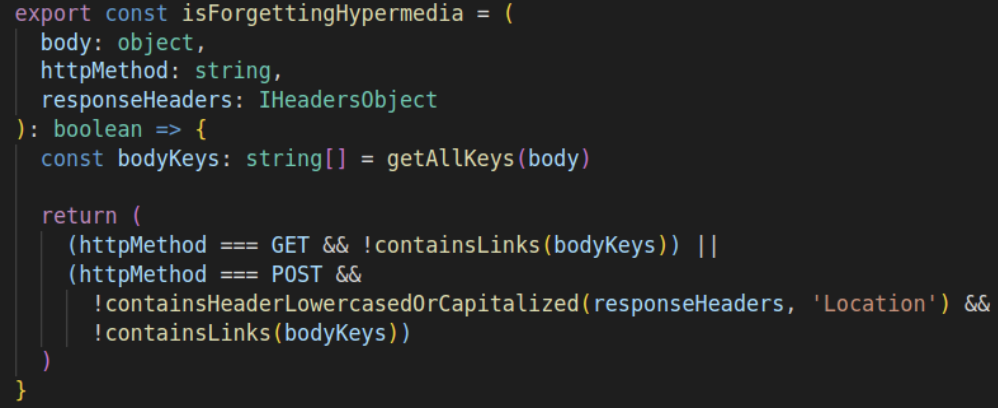
\includegraphics[width=0.8\textwidth]{img/forgettingHyperMedia.png}
 \caption{The detection of Forgetting Hypermedia antipattern.}
 \label{fig:ForgettingHypermedia}
\end{figure}

As shown in Figure \ref{fig:IgnoringCaching}, the Ignoring Caching antipattern gets detected for responses to GET requests if the response headers do not contain an ETag or if the request or response headers does not contain a Cache-Control header or if that is set to `no-cache' or `no-store'.

\begin{figure}[h!]
 \centering
 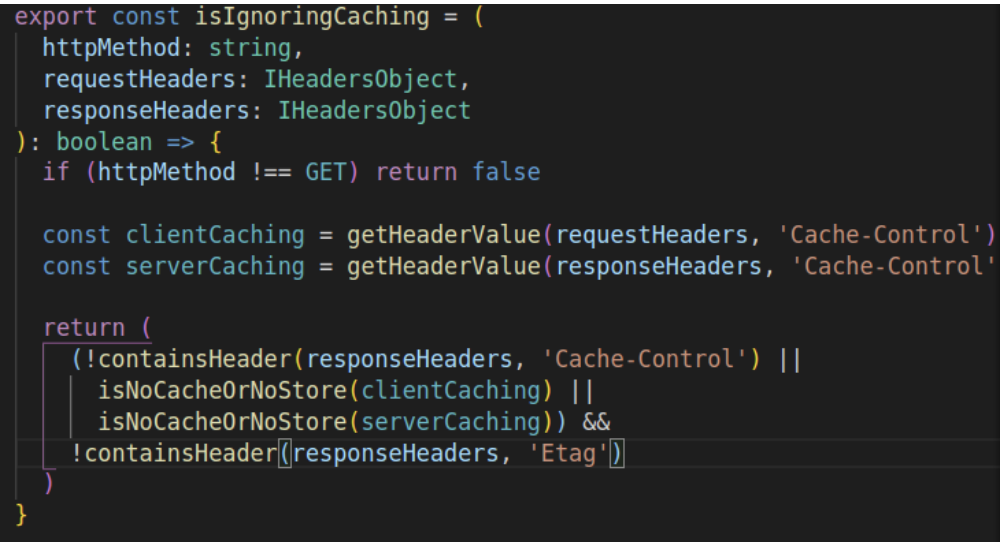
\includegraphics[width=0.8\textwidth]{img/ignoringCaching.png}
 \caption{The detection of Ignoring Caching antipattern.}
 \label{fig:IgnoringCaching}
\end{figure}

As shown in Figure \ref{fig:IgnoringMIMETypes}, the Ignoring MIME Types gets detected if the response Content-Type header's value is not a standard mime type or if it is not among the accepted mime types requested.

\begin{figure}[h!]
 \centering
 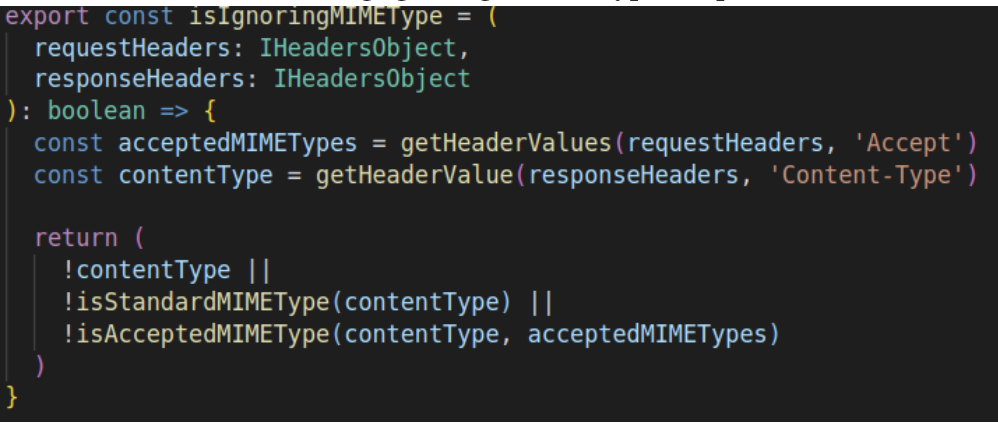
\includegraphics[width=0.8\textwidth]{img/ignoringMimeType.png}
 \caption{The detection of Ignoring MIME Types antipattern.}
 \label{fig:IgnoringMIMETypes}
\end{figure}

As shown in Figure \ref{fig:IgnoringStatusCode}, if the HTTP method used is GET, POST, PUT or DELETE, antipattern Ignoring Status Code gets detected if the combination of HTTP method, status code and status text in the response is not part of a list of valid combinations in an XML file used in the implementation by Palma et al.  \cite{linguistic}.

\begin{figure}[h!]
 \centering
 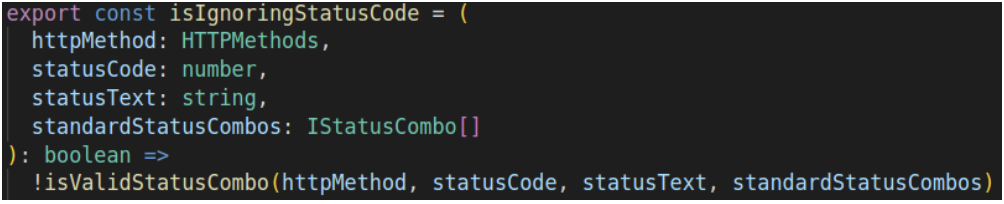
\includegraphics[width=0.8\textwidth]{img/ignoringStatusCode.png}
 \caption{The detection of Ignoring Status Code antipattern.}
 \label{fig:IgnoringStatusCode}
\end{figure}

As shown in Figure \ref{fig:MisusingCookies}, the Misusing Cookies antipattern gets detected if the request or response headers contain any type of cookie header.

\begin{figure}[h!]
 \centering
 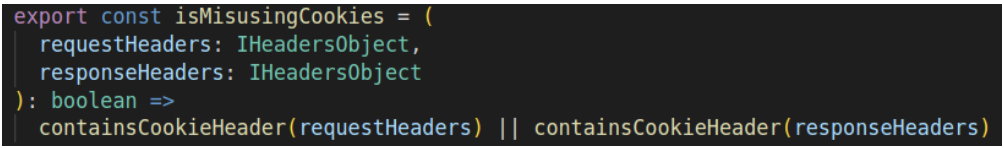
\includegraphics[width=0.9\textwidth]{img/misusingCookies.png}
    \caption{The detection of Misusing Cookies antipattern.}
    \label{fig:MisusingCookies}
\end{figure}

\subsection{Detection of Design Patterns}

After detecting antipatterns and storing meta data about them, this function in Figure \ref{fig:Detectingpatterns} is used to determine and store information about patterns in our Node.js data-handler program. The patterns are set to true, meaning they are fulfilled, if the corresponding antipatterns are set to false, meaning no such antipattern was detected\footnote{\url{https://github.com/rest-api-antipattern-inspector/data-handler}}.

\begin{figure}[h!]
\begin{center}
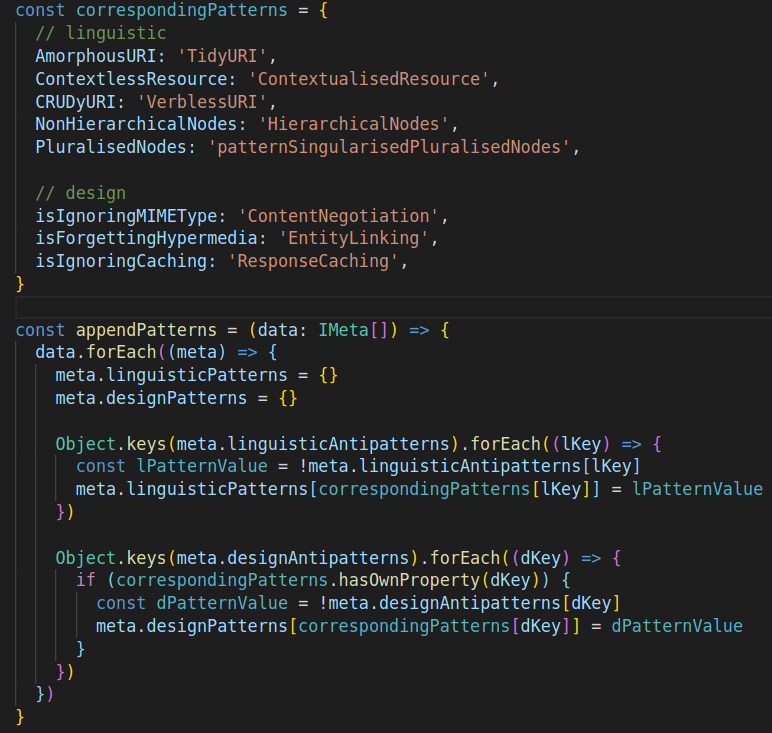
\includegraphics[width=0.75\textwidth]{img/patternsFunction.png}
    \caption{Detecting design patterns.}
    \label{fig:Detectingpatterns}
    \end{center}
\end{figure}

\clearpage

\subsection{Pairwise Phi Coefficient Calculations}

Pairwise Phi Coefficient calculations are made between all design quality aspects and all linguistic quality aspects, this results in a number indicating the strength of the relation between the aspects. This number is between -1 and 1. A Phi Coefficient above 0 indicates a positive relation and one below 0 indicates a negative relation. 0-0.19 indicates a negligible positive relation, 0.2-0.29 a weak positive, 0.3-0.39 a moderate positive and above that is a strong or very strong positive and vice versa is the case for negative numbers indicating the strength of negative relations \cite{phico}. 

Figure \ref{fig:tableComparison} illustrates data used for a Phi Coefficient calculation between the occurrence of two aspects among API endpoints. Figure \ref{fig:phico} shows our implementation in Python for making each pairwise Phi Coefficient comparison calculation\footnote{\url{https://github.com/rest-api-antipattern-inspector/table-phico}}. Variable a is the amount of endpoints where both aspects were detected, b is the amount of endpoints where only the first aspect were detected (CRUDy URIs in the case of figure \ref{fig:tableComparison}), c is the amount of endpoints where only the second aspect were detected (Misusing Cookies in the case of figure \ref{fig:tableComparison} and d is the amount of endpoints where neither of the aspects were detected. 

\begin{figure}[!htb]
    \centering
    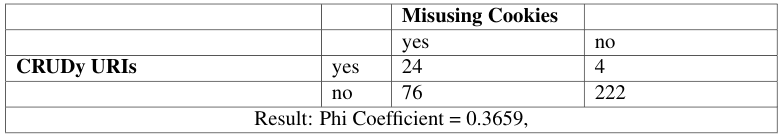
\includegraphics[width=1\textwidth]{img/CRUDy_vs_Cookies.png}
    \caption{Contingency table for comparison of two aspects}
    \label{fig:tableComparison}
\end{figure}

\begin{figure}[!htb]
    \centering
    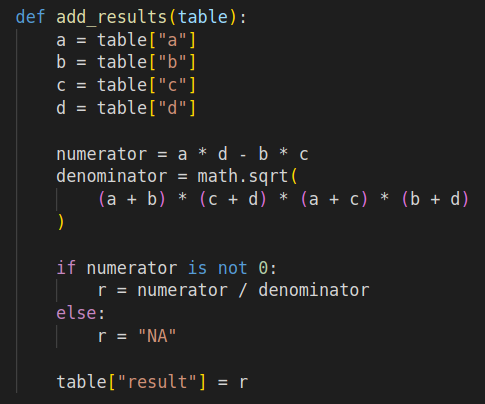
\includegraphics[width=0.6\textwidth]{img/phico.png}
    \caption{Our Phi Coefficient Calculation Implementation in Python}
    \label{fig:phico}
\end{figure}

\newpage